\documentclass[11pt]{article}
\usepackage[margin=0.82in]{geometry}
\usepackage[T1]{fontenc}
\usepackage[utf8]{inputenc}
\usepackage{lmodern}
\usepackage{amsmath,amssymb}
\usepackage{graphicx}
\usepackage{booktabs}
\usepackage{tabularx}
\usepackage{array}
\usepackage{pdflscape}
\usepackage{float}
\usepackage{xcolor}
\usepackage{microtype}
\usepackage{hyperref}
\hypersetup{colorlinks=true,linkcolor=blue!55!black,urlcolor=blue!55!black,citecolor=blue!55!black}
\setlength{\parindent}{0pt}
\setlength{\parskip}{0.55em}

\title{Computational Supplement:\\Correlation Emergence and the Epps Effect}
\author{Chris Angstmann \and Tim Gebbie}
\date{Software release v1.0.0 --- 1 August 2026}

\begin{document}
\maketitle

\begin{abstract}
This supplement records the deterministic computational companion to ``Correlation emergence and the Epps effect in two coupled limit order books'' (arXiv:2606.14182). It evaluates the paper's ordinary and fractional correlation build-up factors, separates clock and coupling components, reports their aggregation-scale sensitivities and identifiability limitations, propagates the local reaction-boundary response into the Epps curve, distinguishes continuum selector regularisation from finite-grid representation error, and supplies a calendar-time bridge with analytical memory diagnostics. The bundle does not simulate the coupled order books, calibrate market data, or treat computational evidence as proof. Its principal purpose is to provide diagnosed analytic curves and a machine-readable interface against which the future v2.0.0 simulation conversion can be overlaid.
\end{abstract}

\tableofcontents

\section{Scientific and software boundary}

The source paper is the mathematical source of truth. The active v1.0.0 route is deliberately narrower than the full coupled reaction--diffusion construction: it evaluates the analytic Epps envelopes and the first-moment response mapping that appear in the paper. The ordinary clock, coupling, and combined curves are illustrations of the stated renewal-envelope, exponential-response, and leading-order separability assumptions. The fractional curves evaluate the stated Mittag--Leffler replacement on the non-negative real axis. The reaction-boundary calculations use only the decaying Gaussian convention for which the paper gives a finite half-line moment.

The following are excluded: empirical covariance estimation; parameter calibration; coupled PDE or order-book path simulation; Monte Carlo validation; the legacy positive-exponential finite-domain source; pointwise equivalence between legacy and regularised couplings; and the Julia-to-Python conversion planned for v2.0.0. In particular, an Epps curve is not treated as sufficient to identify reaction-front thickness or two fractional orders without independent information.

\section{Theory-to-computation map}

The ordinary build-up kernel is
\begin{equation}
F(x)=1-\frac{1-e^{-x}}{x},\qquad x\geq0,
\label{eq:ordinary}
\end{equation}
with (F(0)=0) defined by continuity. The implementation uses \texttt{expm1} away from the origin and the local series
\begin{equation}
F(x)=\frac{x}{2}-\frac{x^2}{6}+\frac{x^3}{24}-\frac{x^4}{120}+O(x^5)
\end{equation}
near zero. Its derivative and local rate elasticity are
\begin{equation}
F'(x)=\frac{1-(1+x)e^{-x}}{x^2},
\qquad
S_F(x)=\frac{xF'(x)}{F(x)}.
\label{eq:elasticity}
\end{equation}

The normalised ordinary components are
\begin{align}
C_{\mathrm{clock}}(\Delta)&=F(\lambda_{12}\Delta),\\
C_{\mathrm{coupling}}(\Delta)&=F(\kappa\Delta),\\
C_{\mathrm{combined}}(\Delta)&=C_{\mathrm{clock}}(\Delta)C_{\mathrm{coupling}}(\Delta).
\end{align}
The last expression is the paper's leading-order factorisation; the calculation does not promote it to an exact independence result.

For a characteristic time \(\tau\), the fractional component is written
\begin{equation}
F_\alpha(\Delta;\tau)
=1-E_{\alpha,2}\!\left[-(\Delta/\tau)^\alpha\right],
\qquad 0<\alpha\leq1.
\label{eq:fractional}
\end{equation}
The release evaluator uses a deterministic real-axis quadrature for \(0<\alpha<1\), a small-argument series, and the exact ordinary formula at \(\alpha=1\). Its planned release profiles are \(\alpha\in\{0.6,0.8,1\}\).

The decaying Gaussian source and its selected half-line moment are
\begin{equation}
q_j(y)=-a_j\mu_j y e^{-\mu_jy^2},
\qquad
M_j^+=\int_0^\infty yq_j(y)\,dy
=-\frac{a_j\sqrt\pi}{4\sqrt{\mu_j}}.
\label{eq:moment}
\end{equation}
The local frozen-front mapping is
\begin{equation}
\kappa_j=\frac{\gamma_{jk}|M_j^+|}{|\mathcal L_j|},
\qquad
\kappa=\kappa_1+\kappa_2.
\label{eq:response}
\end{equation}

\section{Ordinary Epps components and sensitivity}

Figure~\ref{fig:ordinary-components} is the analytic baseline reserved for later simulation overlays. The three panels nondimensionalise the clock rate to one and vary the response-to-clock rate ratio. The curves separate the two mechanisms before forming the combined product.

\begin{figure}[p]
\centering
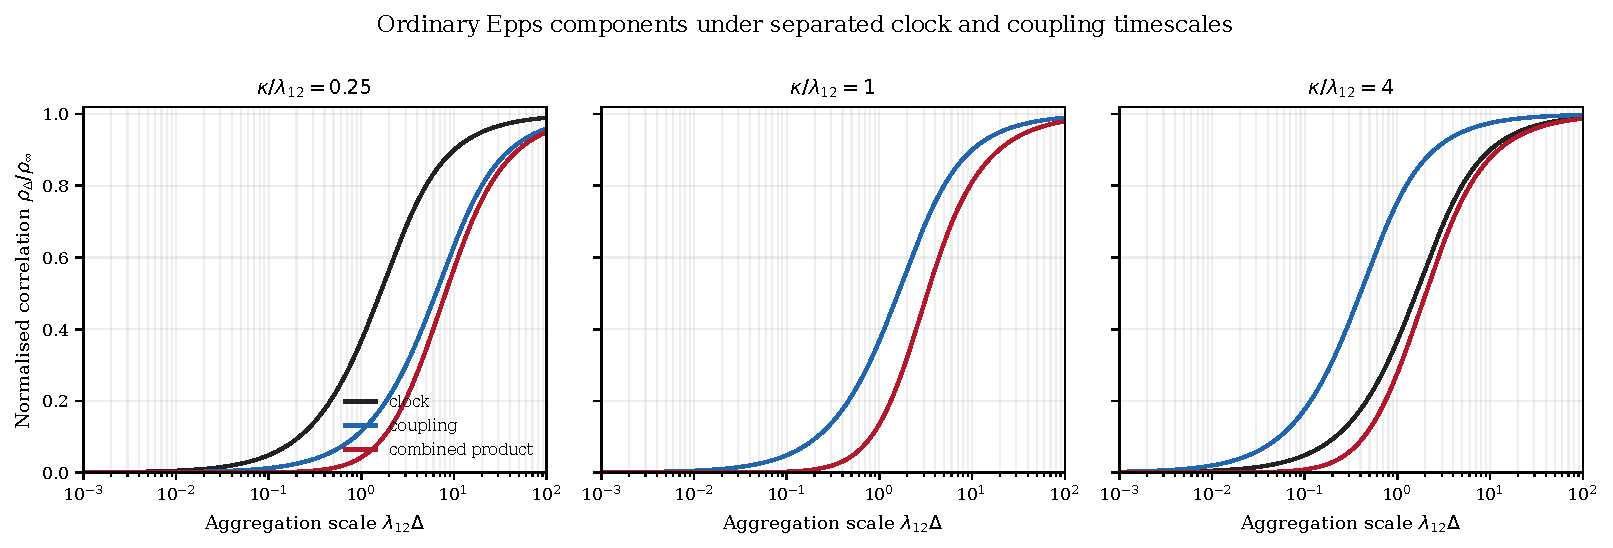
\includegraphics[width=\textwidth]{figures/figure-01-ordinary-epps-components-v1.pdf}
\caption{\textbf{Ordinary Epps components under separated clock and coupling timescales.} The clock curve is $F(\lambda_{12}\Delta)$, the coupling-response curve is $F(\kappa\Delta)$, and the combined curve is their separable product. The horizontal axis is aggregation scale in clock characteristic-time units and the vertical axis is $\rho_\Delta/\rho_\infty$. Panels use $\kappa/\lambda_{12}=0.25,1,4$, with $\lambda_{12}=1$ and $\rho_\infty=1$. The figure shows how the mechanisms contribute across separated and comparable timescales and supplies the analytic overlay baseline for v2.0.0. It supports the component decomposition under the paper's renewal-envelope and separability assumptions; it does not fit market data, simulate an order book, prove statistical independence, or establish the approximation outside those assumptions.}
\label{fig:ordinary-components}
\end{figure}

The short-scale limit of each component is linear in its dimensionless argument, so its rate elasticity approaches one. Once the component reaches its plateau, the elasticity approaches zero. For the product, the partial log-sensitivity to each rate is inherited from that component, while a common proportional perturbation of both rates has the sum of the two partial elasticities.

\begin{figure}[p]
\centering
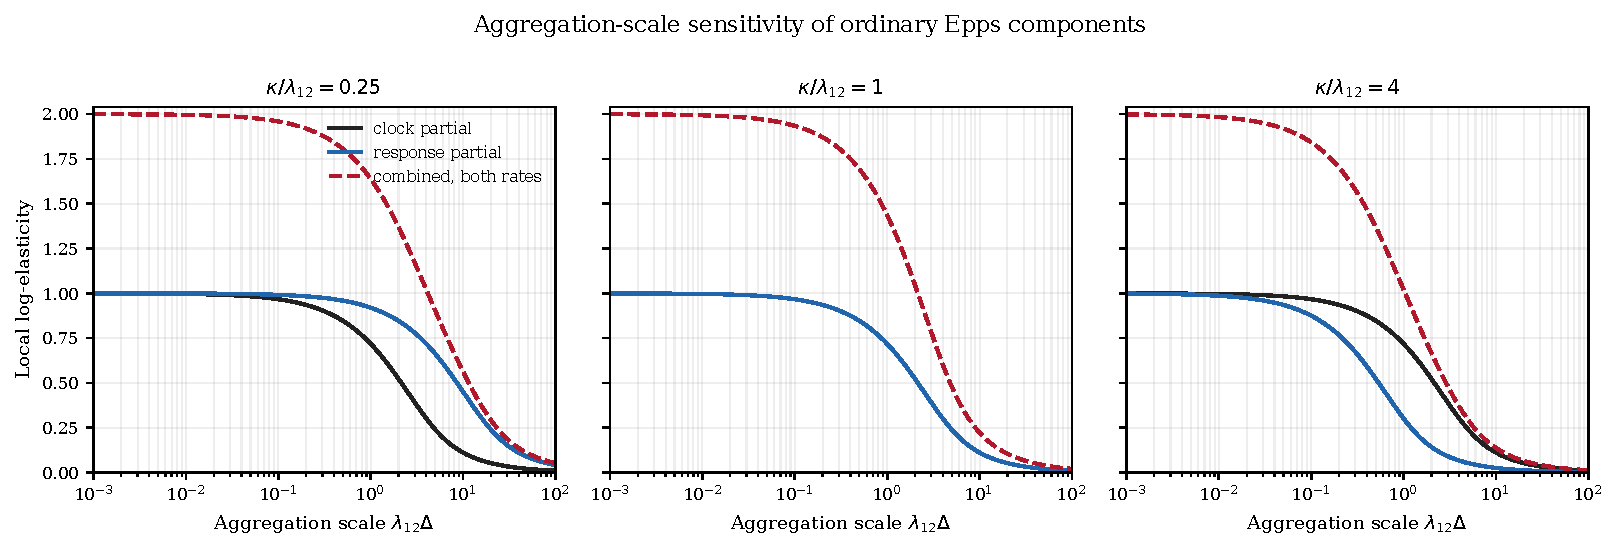
\includegraphics[width=\textwidth]{figures/figure-02-ordinary-epps-sensitivity-v1.pdf}
\caption{\textbf{Aggregation-scale sensitivity of ordinary Epps components.} Curves report $S_F(x)=xF'(x)/F(x)$ for clock refresh and coupling response. The dashed red curve is the log-sensitivity of the combined product when both rates receive the same proportional perturbation. Panels use the Figure~\ref{fig:ordinary-components} rate ratios. Sensitivity tends to one per component in the resolved short-scale limit and to zero on the long-scale plateau, locating the aggregation range that contains rate information. The figure supports local, model-conditional sensitivity statements; it is not a global-identifiability proof, an empirical uncertainty estimate, or evidence that either rate can be recovered without adequate short-scale observations.}
\label{fig:ordinary-sensitivity}
\end{figure}

The combined ordinary curve is invariant under exchange of the clock and response rates. Moreover,
\begin{equation}
C_{\mathrm{combined}}(\Delta)
=\frac{\lambda_{12}\kappa}{4}\Delta^2+O(\Delta^3)
\end{equation}
at short scale. Thus the leading combined curve alone reveals the rate product rather than assigning each timescale to its mechanism. An independently measured refresh rate will be important when interpreting future simulations.

\section{Fractional order sensitivity}

From Eq.~\eqref{eq:fractional},
\begin{equation}
F_\alpha(\Delta;\tau)
=\frac{(\Delta/\tau)^\alpha}{\Gamma(\alpha+2)}
+O(\Delta^{2\alpha}).
\end{equation}
A combined fractional curve therefore has leading power \(\Delta^{\alpha_c+\alpha_r}\). Equal-sum order pairs are deliberately included in Figure~\ref{fig:fractional} to show the resulting local confounding.

\begin{figure}[p]
\centering
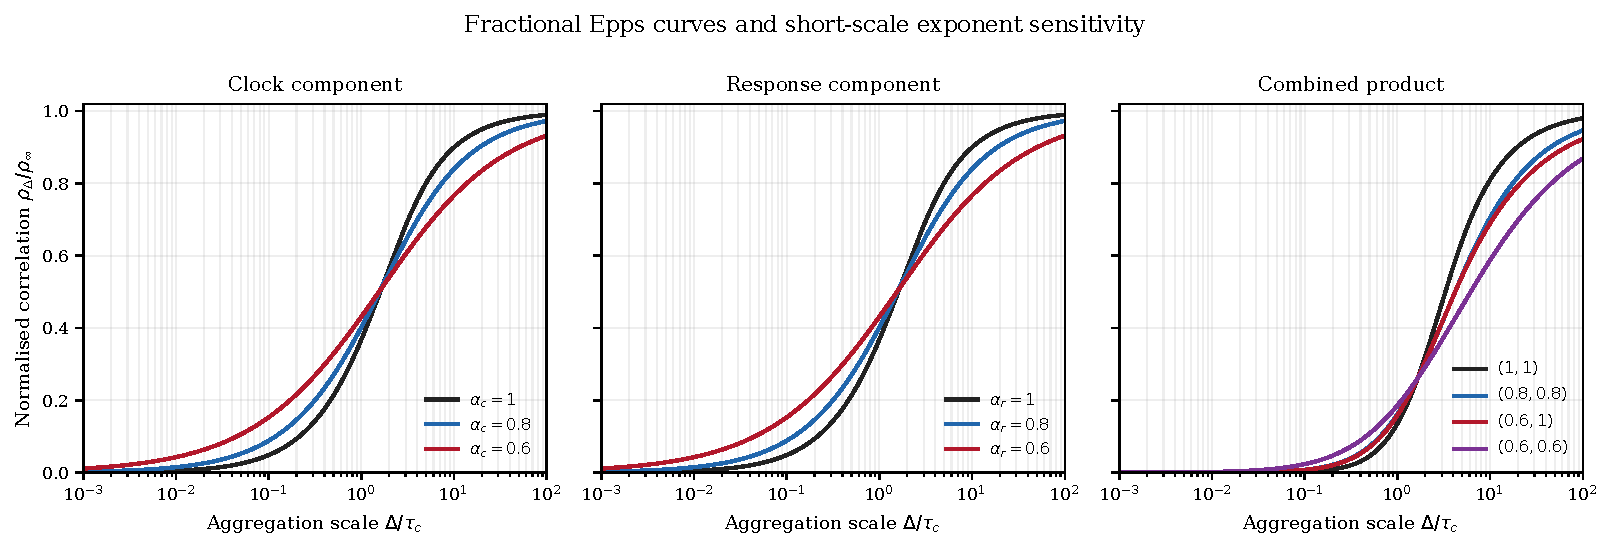
\includegraphics[width=\textwidth]{figures/figure-03-fractional-epps-sensitivity-v1.pdf}
\caption{\textbf{Fractional Epps curves and short-scale exponent sensitivity.} Clock and response components use Eq.~\eqref{eq:fractional}, with unit characteristic times and the diagnosed evaluator recorded in the numerical-design note; \(\alpha=1\) recovers the ordinary kernel. Combined curves use order pairs \((1,1),(0.8,0.8),(0.6,1),(0.6,0.6)\). The equal-sum cases \((0.8,0.8)\) and \((0.6,1)\) share leading short-scale power \(\Delta^{1.6}\), exposing local confounding even when later-scale curvature differs. The figure shows formula sensitivity to fractional order and the ordinary limit. It does not identify both orders from a combined curve alone, attach an unconditional ``slower'' interpretation across dimensional conventions, or validate a fractional market-clock mechanism empirically.}
\label{fig:fractional}
\end{figure}

\section{Conditional reaction-boundary propagation}

Equation~\eqref{eq:response} yields conditional log-elasticities $+1,+1,-1/2,-1$ with respect to coupling strength, source amplitude, source width, and front-slope magnitude. Figure~\ref{fig:boundary} changes one quantity at a time. This is a propagation experiment: multiple structural parameter combinations generate the same effective response rate and hence the same analytic Epps curve.

\begin{figure}[p]
\centering
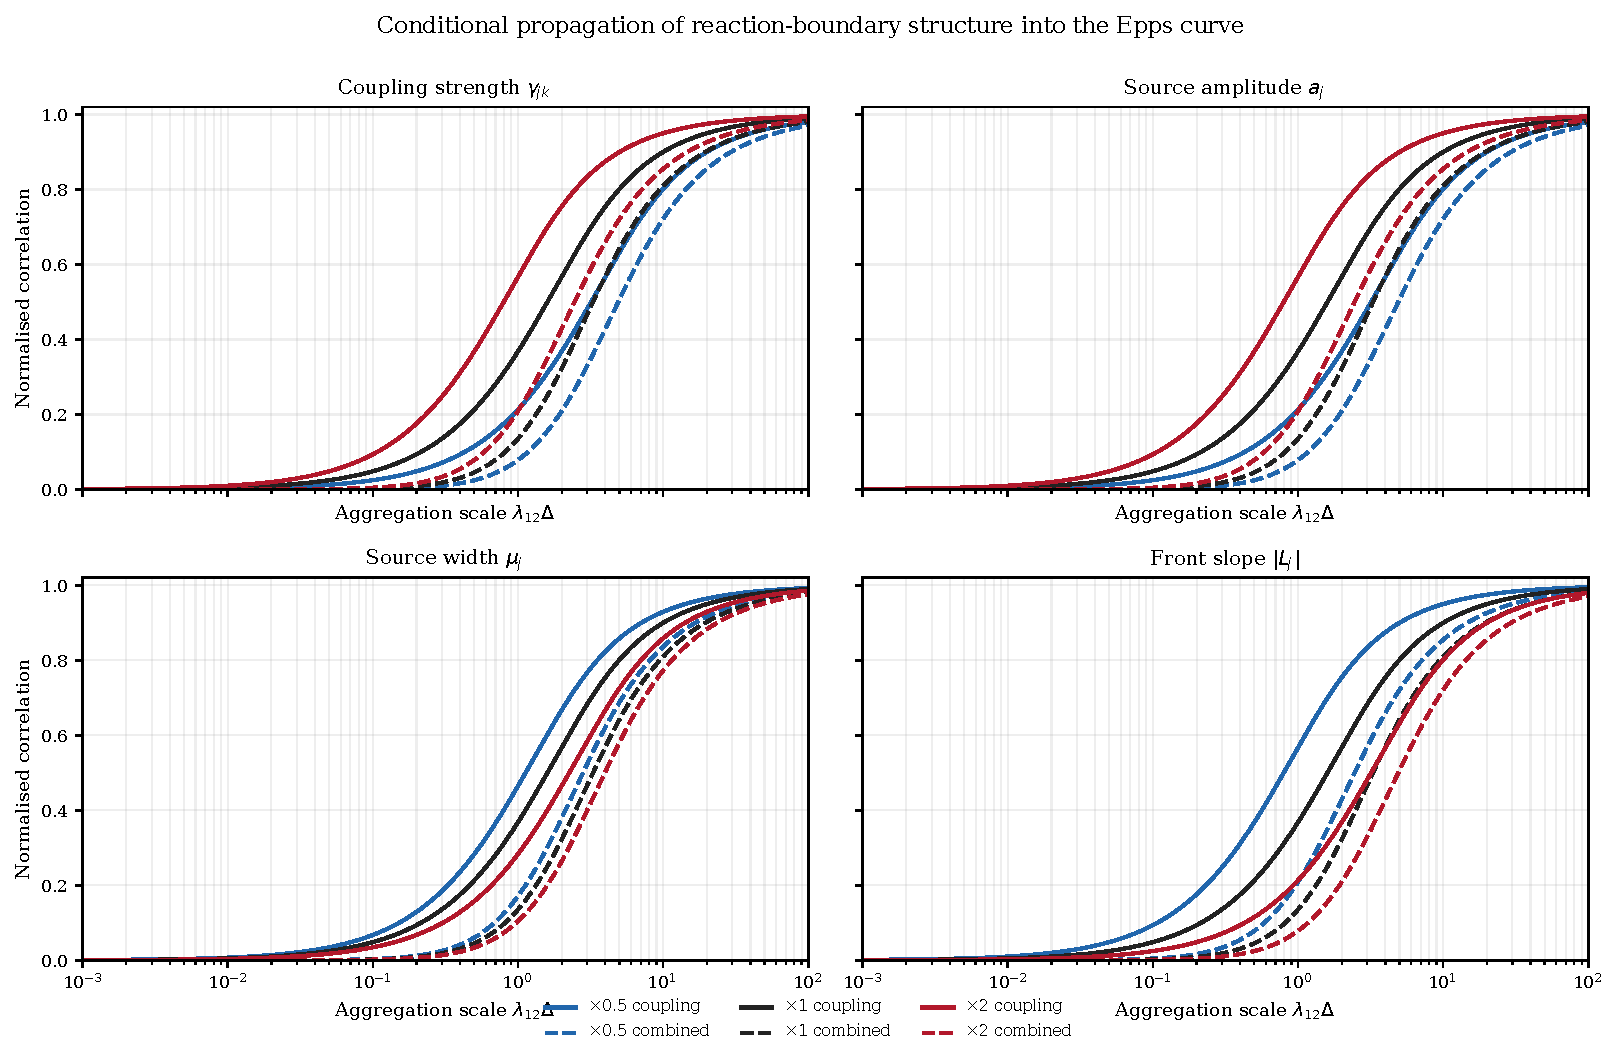
\includegraphics[width=\textwidth,height=0.72\textheight,keepaspectratio]{figures/figure-04-boundary-to-epps-propagation-v1.pdf}
\caption{\textbf{Conditional propagation of reaction-boundary structure into the Epps curve.} The response rate is varied through Eqs.~\eqref{eq:moment}--\eqref{eq:response}. Two symmetric books, unit source amplitude, width and front-slope magnitude, and $\gamma_{jk}=2/\sqrt\pi$ give baseline total response rate $\kappa=1$. Each panel changes one input by factors $0.5,1,2$, holding the others and the unit clock rate fixed; solid curves are coupling factors and dashed curves their combined products with the clock factor. This supports conditional propagation through the analytic response mapping. It does not uniquely infer reaction-front thickness, source width, or coupling strength from an Epps curve and does not claim pointwise equivalence to the legacy lattice coupling.}
\label{fig:boundary}
\end{figure}

Three distinct notions must not be collapsed into a single ``boundary thickness'': the local reaction-front slope \(|\mathcal L_j|\), the continuum selector regularisation \(\varepsilon\), and the lattice spacing \(\Delta x\). The first enters the structural response mapping. The second regularises side selection. The third is a numerical resolution parameter.

\section{Continuum selector and finite-grid representation}

The paper's smooth selector is
\begin{equation}
W(y,z;\varepsilon)=\frac12\left[1+\tanh\left(\frac{yz}{\varepsilon}\right)\right].
\end{equation}
For a centred symmetric full domain, \(yq_j(y)\) is even and the hyperbolic-tangent contribution is odd. Consequently the selected first moment is independent of \(\varepsilon\) in the continuum calculation. Finite domains, misaligned numerical selectors, and coarse grids can break this cancellation. Figure~\ref{fig:grid} diagnoses those representation effects and propagates them through an effective response rate.

\begin{figure}[p]
\centering
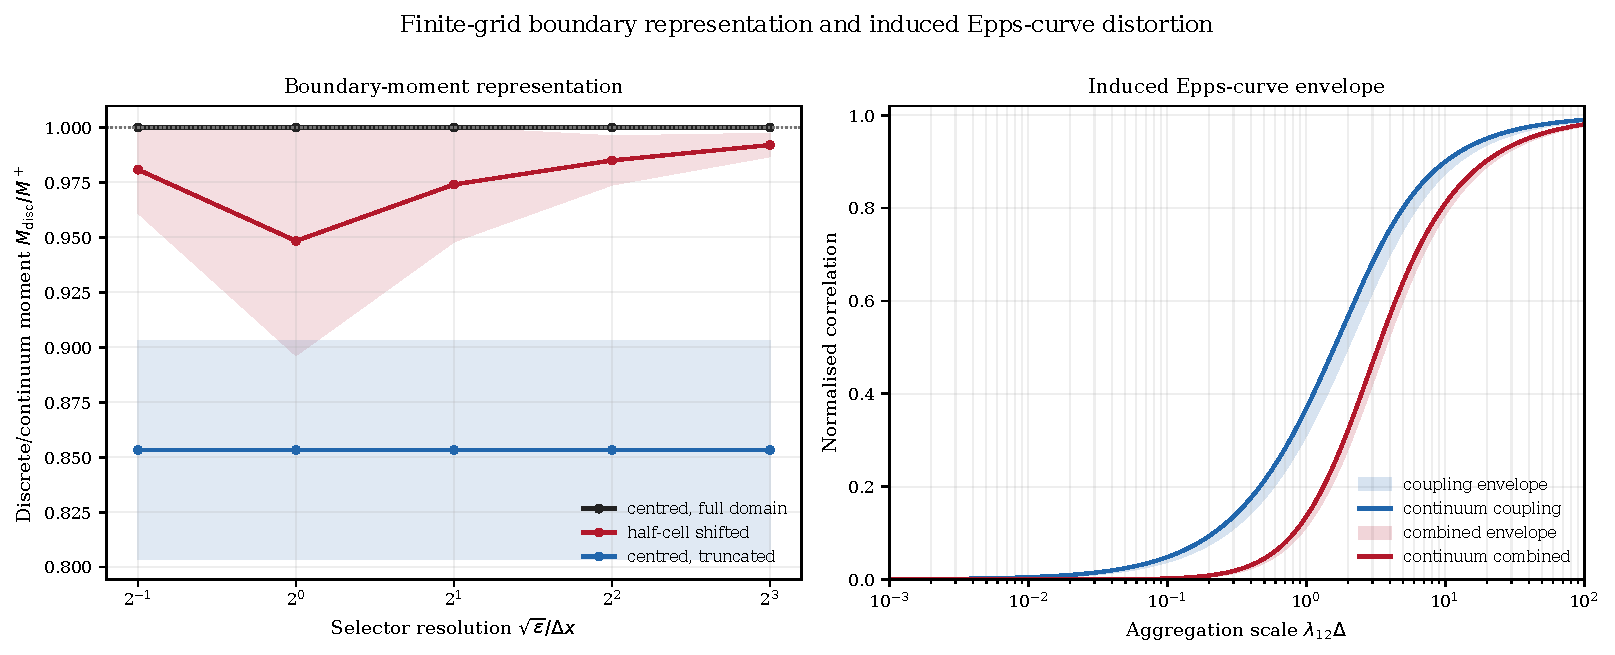
\includegraphics[width=\textwidth]{figures/figure-05-finite-grid-epps-distortion-v1.pdf}
\caption{\textbf{Finite-grid boundary representation and induced Epps-curve distortion.} The left panel reports discrete-to-continuum first-moment ratios as selector resolution \(\sqrt\varepsilon/\Delta x\), lattice spacing, selector alignment, and domain margin vary. Lines give the midpoint and bands the range over four lattice spacings. The centred full-domain case is the parity control; half-cell selector displacement and truncation measure numerical representation errors. The right panel propagates all diagnosed effective-rate ratios through the coupling and combined Epps formulas; lines are continuum baselines and bands are discrete-representation envelopes. Structural parameters are fixed. The figure supports convergence and numerical-sensitivity statements and defines resolution metadata required for v2 overlays. It does not introduce a new continuum Epps mechanism or treat selector width, lattice spacing, and reaction-front thickness as interchangeable.}
\label{fig:grid}
\end{figure}

\clearpage
\section{Calendar-time representation and memory diagnostic}

The aggregation variable in Figures~\ref{fig:ordinary-components}--\ref{fig:grid} remains the observation-window lag, but is reported relative to the clock characteristic time. Writing
\begin{equation}
x=\lambda_{12}\Delta t=\frac{\Delta t}{\tau_c},
\qquad \tau_c=\lambda_{12}^{-1},
\end{equation}
shows that a calendar-time presentation requires only a declared time convention. For an ordinary exponential memory with rate \(r\),
\begin{equation}
h_r(u)=e^{-ru},
\qquad
F(r\Delta t)=1-\frac{1}{\Delta t}\int_0^{\Delta t}h_r(u)\,du.
\label{eq:memory-average}
\end{equation}
For the clock mechanism, \(h_{\lambda_{12}}\) is the no-refresh survival. For the coupling mechanism, \(h_\kappa\) is the relaxation survival and equals the normalised positive-lag exponential covariance kernel used in the paper. Figure~\ref{fig:calendar-bridge} therefore presents the same analytical factors as Figure~\ref{fig:ordinary-components}, not a new Epps mechanism.

\begin{figure}[p]
\centering
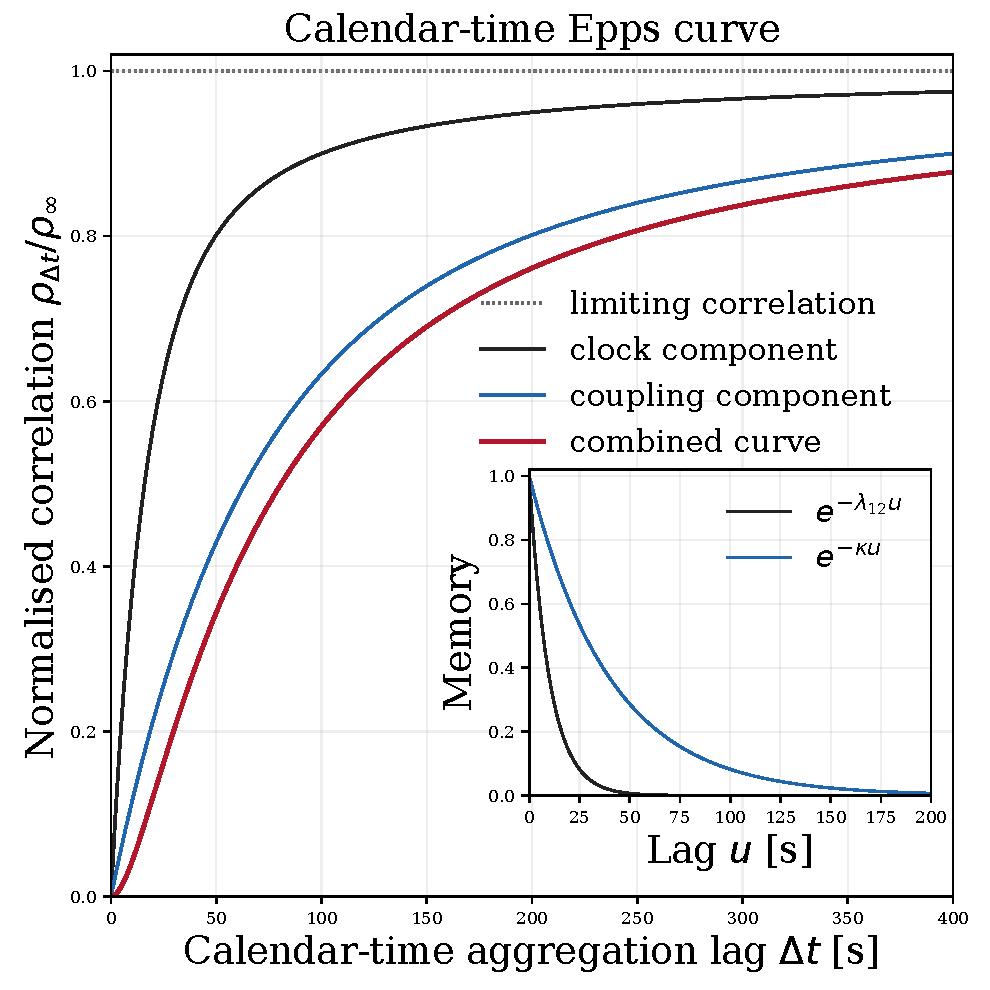
\includegraphics[width=0.91\textwidth]{figures/figure-06-calendar-time-epps-memory-v1.pdf}
\caption{\textbf{Calendar-time Epps curve.} The square main panel rewrites the Figure~\ref{fig:ordinary-components} slow-response profile on a linear calendar-time axis using the explicitly illustrative convention $\lambda_{12}=0.1\,\mathrm{s}^{-1}$, $\kappa=0.025\,\mathrm{s}^{-1}$, and $\rho_\infty=1$, corresponding to $\tau_c=10$ s and $\tau_r=40$ s. Black, blue and red curves are the clock factor, coupling factor and their leading-order separable product; the grey dotted line marks the normalised limiting correlation $\rho_{\Delta t}/\rho_\infty=1$. The enlarged inset reports $h_c(u)=e^{-\lambda_{12}u}$ and $h_r(u)=e^{-\kappa u}$: respectively the no-refresh survival and coupling relaxation survival, with the latter also equal to the normalised positive-lag exponential covariance kernel. The figure shows that the conventional calendar-time Epps presentation is a dimensional re-expression of the same analytical build-up factors. The seconds scale is not fitted to data, and the inset is neither a path autocorrelation nor a power-spectrum estimate. Those path-derived diagnostics are reserved for v2.0.0.}
\label{fig:calendar-bridge}
\end{figure}

The distinction from the future simulation output is substantive. A simulated power spectrum or sample autocorrelation requires a generated price path and an estimator, together with finite-sample and iteration uncertainty. None exists in v1.0.0. The deterministic inset instead exposes the memory functions that enter Eq.~\eqref{eq:memory-average}; a path-derived spectral inset may be added alongside the simulation curve in v2.0.0 without retrospectively relabelling this analytical diagnostic.

\clearpage
\begin{landscape}
% Standalone table fragment. Required packages: booktabs, tabularx, array, float.
\begin{table}[H]
\centering
\scriptsize
\caption{\textbf{Parameter, timescale and identifiability register.} The table maps paper notation to implementation names and records units, roles, sensitivity pathways, and fixed or swept status. Refresh rate and source amplitude receive different code names despite source-notation overlap. Identifiability classifications describe the information available from the planned outputs under the stated model; they are not estimates, formal statistical-identifiability proofs, or empirical calibration results.}
\label{tab:parameter-register}
\renewcommand{\arraystretch}{0.98}
\begin{tabularx}{\linewidth}{@{}p{1.7cm}p{3.3cm}p{2.3cm}p{2.5cm}X X X X@{}}
\toprule
Paper symbol & Code name & Source & Units & Role & Sensitivity path & Figure treatment & Identifiability from Epps output \\
\midrule
\(\Delta\) & \texttt{aggregation\_\allowbreak{}scale} & Eqs. (8), (9), (11) & time; dimensionless after scaling & return aggregation horizon & direct horizontal scale & swept in F1-F6 & observed/design variable \\
\(\rho_\infty\) & \texttt{rho\_\allowbreak{}inf} & Eqs. (8), (9), (11) & dimensionless correlation & long-scale vertical level & multiplicative vertical scale & fixed to one in base figures & conditional on plateau coverage \\
\(\lambda_{12}\) & \texttt{clock\_\allowbreak{}rate} & Eq. (8); App. A & time\(^{-1}\) & pooled refresh/overlap rate & \(F(\lambda_{12}\Delta)\) & unit scale; sensitivity in F2 & conditional; independently measurable in v2 \\
\(\kappa=\kappa_1+\kappa_2\) & \texttt{response\_\allowbreak{}rate} & Eq. (9); App. B & time\(^{-1}\) & spread relaxation rate & \(F(\kappa\Delta)\) & swept in F1-F2; derived in F4-F5 & conditional on clock rate and short scales \\
\(\alpha_c\) & \texttt{alpha\_\allowbreak{}clock} & App. C, Eq. (C.18) & dimensionless & fractional clock order & short power \(\Delta^{\alpha_c}\) & swept in F3 & not separate from alpha\_response at short scale \\
\(\alpha_r\) & \texttt{alpha\_\allowbreak{}response} & App. C, Eq. (C.18) & dimensionless & fractional response order & short power \(\Delta^{\alpha_r}\) & swept in F3 & not separate from alpha\_clock at short scale \\
\(\tau_c,\tau_r\) & \texttt{clock\_\allowbreak{}characteristic\_\allowbreak{}time}\newline\texttt{response\_\allowbreak{}characteristic\_\allowbreak{}time} & v1 nondimensionalisation & time & fractional scale convention & \((\Delta/\tau)^\alpha\) & fixed to one in F3 & confounded with fractional rate convention \\
\(\gamma_{jk}\) & \texttt{coupling\_\allowbreak{}strength} & Eq. (6); App. B & model-dependent & pair-trader coupling strength & \(\kappa_j\propto\gamma_{jk}\) & one-at-a-time sweep in F4 & not separate from source/front quantities \\
\(\lambda_j\) (source) & \texttt{source\_\allowbreak{}amplitude} & Eq. (5); App. B & source amplitude & decaying-Gaussian amplitude & \(M_j^+\propto a_j\) & one-at-a-time sweep in F4 & not separate from coupling strength \\
\(\mu_j\) & \texttt{source\_\allowbreak{}width} & Eq. (5); App. B & price\(^{-2}\) & Gaussian source-shape scale & \(M_j^+\propto\mu_j^{-1/2}\) & one-at-a-time sweep in F4 & not separate from amplitude/front slope \\
\(|\mathcal L_j|\) & \texttt{front\_\allowbreak{}slope\_\allowbreak{}abs} & Eq. (B.9); Eq. (B.13) & density per price & frozen reaction-front slope & \(\kappa_j\propto|\mathcal L_j|^{-1}\) & one-at-a-time sweep in F4 & not identifiable as thickness from Epps alone \\
\(\varepsilon\) & \texttt{epsilon} & Eq. (6); App. D & price\(^2\) for \(yz/\varepsilon\) & continuum selector regularisation & centred moment invariant; representation path & swept in F5 & not a reaction-front thickness parameter \\
\(\Delta x\) & \texttt{lattice\_\allowbreak{}spacing} & App. D & price & numerical lattice resolution & discrete moment error to effective response & swept in F5 & known numerical control \\
\(z_{jk}\) & \texttt{directed\_\allowbreak{}spread} & Eq. (6); App. B & price & directed book-price spread & selector argument \(yz/\varepsilon\) & fixed to 0.2 in F5 & state variable, not inferred parameter \\
-- & \texttt{alignment\_\allowbreak{}offset\_\allowbreak{}cells} & v1 numerical diagnostic & lattice cells & source-selector centring error & parity breaking to effective response & 0 and 0.5 in F5 & known numerical control \\
-- & \texttt{domain\_\allowbreak{}halfwidth} & v1 numerical diagnostic & price & finite integration/lattice domain & tail truncation to effective response & full and truncated in F5 & known numerical control \\
\bottomrule
\end{tabularx}
\end{table}

\end{landscape}

\begin{landscape}
% Standalone table fragment. Required packages: booktabs, tabularx, array, float.
\begin{table}[H]
\centering
\scriptsize
\caption{\textbf{Numerical benchmarks, convergence tests and acceptance status.} Each row records a claim-relevant diagnostic, its analytic or independent reference result, declared tolerance, observed value or error, and acceptance status. Checks cover the ordinary kernel and derivative, fractional $\alpha=1$ recovery and independent reference values, the decaying-Gaussian first moment, centred-selector invariance, finite-grid refinement, invalid inputs, and the analytic/simulation overlay contract. The table supports numerical reliability and reproducible execution within the tested environment; it is not a mathematical proof of the model, an empirical validation, or evidence for excluded legacy-simulation claims.}
\label{tab:numerical-benchmarks}
\renewcommand{\arraystretch}{1.02}
\begin{tabularx}{\linewidth}{@{}p{0.9cm}p{3.6cm}X p{3.0cm}X p{1.8cm}@{}}
\toprule
ID & Diagnostic & Expected result & Tolerance & Observed result & Status \\
\midrule
D01 & Ordinary zero and small-argument limit & F(0)=0 and the declared small-x series is recovered & abs error <= 1.0e-12 & F(0)=0.000e+00; series error at 1e-6=0.000e+00 & Verified \\
D02 & Ordinary bounds and monotonicity & 0 <= F(x) < 1 and non-decreasing for x >= 0 & violation <= 1.0e-12 & range=[0.00000500, 0.99000000]; min increment=1.641e-07 & Verified \\
D03 & Ordinary analytic derivative & Analytic derivative agrees with centred finite differences & max error <= 2.0e-07 & max error=2.084e-10 & Verified \\
D04 & Ordinary elasticity limits & S\_F -> 1 at short scale and S\_F -> 0 at long scale & combined limit error <= 2.0e-05 & S(1e-8)=0.999999996667; S(1e5)=1.000e-05 & Verified \\
D05 & Fractional alpha-one recovery & F\_alpha with alpha=1 equals the ordinary kernel & max error <= 2.0e-13 & max error=0.000e+00 & Verified \\
D06 & Fractional independent reference values & Release evaluator matches adaptive-quadrature references & max error <= 2.0e-09 & six-point max error=1.571e-13 & Verified \\
D07 & Fractional bounds and monotonicity & Release curves remain in [0,1] and non-decreasing & violation <= 2.0e-09 & maximum violation=0.000e+00 & Verified \\
D08 & Decaying-Gaussian first moment & Numerical full-domain selected moment equals analytic half-line moment & relative error <= 2.0e-06 & analytic=-0.443113462726; numerical=-0.443113462726 & Verified \\
D09 & Centred-selector continuum invariance & Symmetric first moment is independent of selector width & relative error <= 2.0e-06 & max relative error over three epsilon values=2.220e-16 & Verified \\
D10 & Centred finite-grid convergence & Moment error decreases from a deliberately coarse lattice under refinement & finest error <= 2.0e-05 & errors=1.935e-01,1.939e-03,1.635e-06,1.110e-15 & Verified \\
D11 & Boundary baseline response normalisation & Two-book baseline total response rate equals one & abs error <= 1.0e-12 & kappa\_total=1.000000000000 & Verified \\
D12 & Combined-factor construction & Combined curve equals diagnosed component product and remains bounded & violation <= 1.0e-12 & range=[0.00000025, 0.98010000] & Verified \\
D13 & Invalid-input handling & Four invalid parameter cases fail clearly & all four raise ValueError & caught=4/4 & Verified \\
D14 & v2 analytic/simulation overlay contract & Required scientific and provenance roles are declared & all ten roles present & declared roles=10/10 & Verified \\
\bottomrule
\end{tabularx}
\end{table}

\end{landscape}

\section{Parameter and numerical evidence}

Table~\ref{tab:parameter-register} keeps the source notation, unambiguous code names, units, sensitivity paths, and identifiability qualifications together. In particular, the paper's refresh-rate and source-amplitude uses of \(\lambda\) are separated in code. Table~\ref{tab:numerical-benchmarks} is generated from the diagnostic results; scientific figures are not accepted if a row is failed. The fractional reference points were computed independently with adaptive quadrature, while the release evaluator uses fixed composite Gauss--Legendre quadrature and a small-argument series.

\section{Reproducibility and the v2 interface}

The complete active route is
\begin{verbatim}
python scripts/run_all.py
\end{verbatim}
and the standard-library regression tests are
\begin{verbatim}
python -m unittest discover -s tests -v
\end{verbatim}
The run regenerates the six PDF/PNG figures, two CSV/LaTeX table pairs, six long-form figure datasets, the shared analytic overlay CSV, diagnostic reports, and this supplement's dependencies. PDF bytes can differ across systems because of renderer metadata or font embedding; machine-readable values and diagnostic statuses are the cross-platform reproducibility objects.

The file \texttt{outputs/epps-overlay-v1.csv} records aggregation scale and unit, curve type, mechanism, normalised and absolute correlation, uncertainty placeholders, parameter profile, and software version. Version 2.0.0 may add simulation rows and uncertainty values without redefining these fields. Simulation resolution, alignment, and domain metadata must accompany any overlay because Figure~\ref{fig:grid} shows that numerical boundary representation can move the apparent response curve.

\section{Interpretive limits}

The diagnosed computations support six limited conclusions. First, the ordinary clock and coupling factors are distinguishable when their timescales are sufficiently separated and the components are shown explicitly. Second, the long-scale plateau contains little local information about either rate. Third, the leading short-scale power of a combined fractional curve identifies an order sum rather than two separate orders. Fourth, reaction-boundary quantities affect the Epps curve conditionally through the effective response rate, but are not individually identified by that curve. Fifth, continuum selector invariance can coexist with finite-grid distortion when parity, alignment, or domain controls are not respected. Sixth, the conventional calendar-time Epps plot is obtained by assigning units to the same aggregation lag, while path autocorrelation and spectral diagnostics require the future simulator.

These are computational illustrations and numerical verification statements inside the paper's assumptions. They are not empirical validation, calibration, proof of the approximations, or evidence that the future converted simulator will reproduce the analytic curves without further checking.

\medskip
\noindent\textbf{Software and licensing note.} Code is provided under the MIT License; supplementary text, captions, generated figures, tables, and documentation are provided under CC BY 4.0. The paper and frozen source retain their existing terms.

\end{document}
